\section{Simultaneous Localization and Mapping}
\label{slam}

Simultaneous Localization and Mapping (SLAM) is a technique for estimating the motion of the robot and reconstructing the map/structure of the unknown environment. SLAM using only visual information only is specifically referred to as visual SLAM (vSLAM). The SLAM problem can be stated as follows:\\

\textbf{\emph{How can a body navigate in a previously unknown environment while constantly building and updating a map of its workspace using onboard sensors only?} [7]}\\

From the problem statement above, we notice that the robot has no a priori knowledge of the workspace or environment that it is in. This makes SLAM a very challenging problem in probabilistic robotics. Accurate pose estimation is critical for many applications in computer vision, autonomous robotics and augmented reality.
  

% For one-column wide figures use
\begin{figure}
% Use the relevant command to insert your figure file.
% For example, with the graphicx package use
  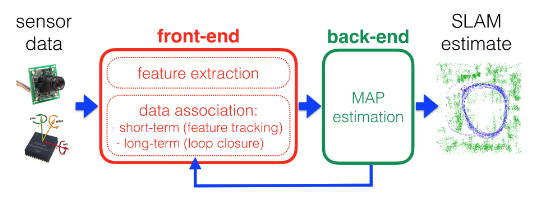
\includegraphics[width=\textwidth]{./figures/slam_model.png}
% figure caption is below the figure
\caption{SLAM architecture}
\label{fig:slammodel}       % Give a unique label
\end{figure}

\subsection{Visual Odometry}

As described in the above section, Odometry is the technique of estimating the position of a robot over time using sensors such as cameras,  wheel encoders or any sensor measuring relative movement. Compared to SLAM which maintains a global consistent map, visual odometry (VO) maintains a local consistent map optimized over the last n frames. A generalized VO pipeline can be summarized as follows

% For one-column wide figures use
\begin{figure}[!htb]
% Use the relevant command to insert your figure file.
% For example, with the graphicx package use
  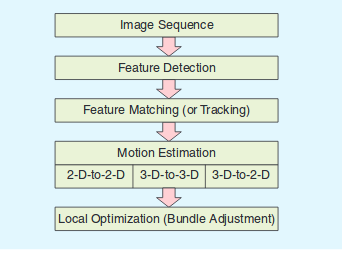
\includegraphics[width=\textwidth]{./figures/vo.png}
% figure caption is below the figure
\caption{Generalized Visual Odometry Pipeline}
\label{fig:vo}       % Give a unique label
\end{figure}

Different algorithms exist due to the different type of cameras available such as Stereo, Mono, RGB-D. As we use a monocular setup in our research paper, we would be going through the visual odometry algorithm from 2D to 2D correspondences for a monocular sensor. The algorithm is summarized as follows.

\begin{algorithm}
    \caption{Monocular Visual Odometry}
	\begin{algorithmic}[1]
		\State Capture a new image frame $I_k$
    	\State Extract and match features between frames $I_k$ and $I_{k-1}$
    	\State Compute the essential matrix $E$ from the matched feature points
    	\State Decompose $E$ into $R_k$ and $t_k$ to form $T_k$
    	\State Choose the correct $T_k$ matrix and scale $t_k$ accordingly from scale factor
    	\State Compute $C_k$ = $C_{k-1}*T_k$
    	\State Goto step 1.
	\end{algorithmic}
\end{algorithm}

Since we are using a monocular sensor, we always compare the image $I_k$ captured at time instant $k$ with the image $I_{k-1}$ capture at time instant $k-1$. In a stereo setup, we would compare images from the left and right part of the stereo. Once an image is captured, we compute the features for image $I_k$ and $I_{k-1}$. In the feature detection step, the image is searched for key-points called features  which are likely to be present in successive images. Features can be defined as image patterns that differ from its immediate neighborhood in terms of intensity, color and texture. There exist a variety of feature detectors in literature which vary in performance and properties. Some of the properties of feature detectors are rotation, scale and affine invariant, repeatability, localization accuracy, robustness and efficiency.  Heitanen et al. present a comparison of feature detectors and descriptors for object class matching in~\cite{hietanen2016comparison}. Once we detect features, we then need to compute a descriptor such that features detected in two images can be compared with each other. The easiest approach would be to form a patch of pixels and compare using a sum of squared distances (SSD) or normalized cross correlation (NCC) metric. Such descriptors are not invariant to any of the above mentioned properties and perform poorly in practical applications. One of the popular descriptors called SIFT~\cite{lowe2004distinctive} uses gradient orientations as its descriptors. This forms a 128-element descriptor that is invariant to most of the above mentioned properties such as rotation, scale and illumination which makes it widely applicable in practical real-time applications. For extracting features from two images there are two paths with one being to detect and match features independently in two frames and the other being to track features in subsequent frames an example of which is a KLT Tracker~\cite{tomasi1991detection}. There are various methods employed to match features accurately such a RANSAC which stands for Random Sample Consensus and is used to remove outliers among feature matches. Once we detect and match features in $I_k$ and $I_{k-1}$, we calculate the essential matrix $E$ which describes the geometric relationship between two images. We can use Nister’s five point algorithm~\cite{nister2004efficient} or Longuet-Higgins eight point algorithm~\cite{longuet1981computer} to get the essential matrix $E$. Once we get the essential matrix $E$, we decompose it to extract the rotation and translation parts. Four different solutions are obtained of which the correct pair can be found out by triangulation. The solutions are given as

\begin{equation}
	R = U(\pm W^T)V^T
\end{equation}

\begin{equation}	
	t = U(\pm W^T)SV^T
\end{equation}

where R is the rotation matrix and t is the translation vector. 

\subsection{EKFSLAM}

\subsection{PTAM}
